\section{Discussions}
\label{sec:discussion}

In this section, we describe the insights we accumulated through ADVISe.

\subsection{Trends}

\subsubsection{Stable enzyme annotations}

The most common event spread over the entire data set is located at the bottom left corner of each frame and represents pairs of observed EC numbers that remained unchanged in pair of releases. It means that the two EC numbers involved were equal (i.e. 3.1.3.2 to 3.1.3.2) or that there was no EC number (i.e. -.-.-.- to -.-.-.-). 

In Figure \ref{fig:heatmap011}, we present a more realistic view of the dataset, aggregating stable entries (subframe (0, 0) at each frame) and changes in other subframes with global normalization and normal scale. We can see there is a global predominance of entries with no generalization or specialization and prefix length 0. These entries usually have undefined EC numbers (-.-.-.-) that remained like so. Notice that the area of this specific subframe is clearly growing across releases what reflects the growth in UniProt/SwissProt database over the fifteen analyzed releases.

In Figure \ref{fig:heatmap010}, we show the same data normalized by frame, what reveals stable entries are predominant in almost every frame. Exceptions do exist and they are going to be discussed in section \ref{sec:exceptions}.

\begin{figure*}[htb]
  \centering
  %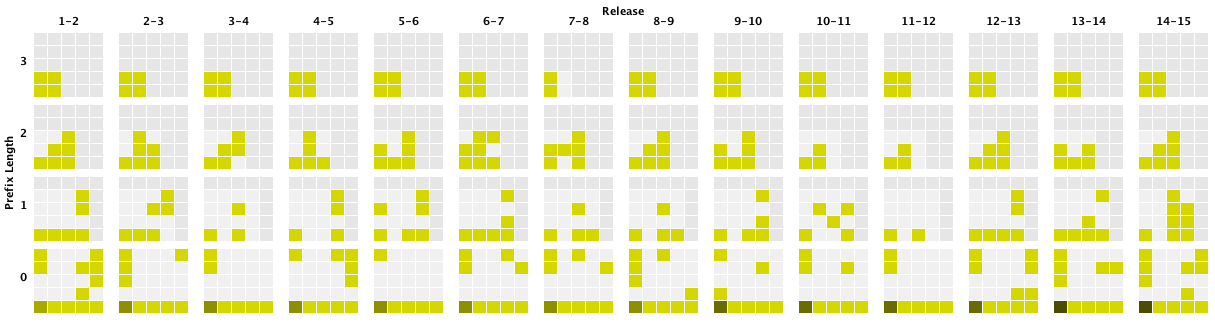
\includegraphics[width=17cm]{images/heatmap011.png} 
  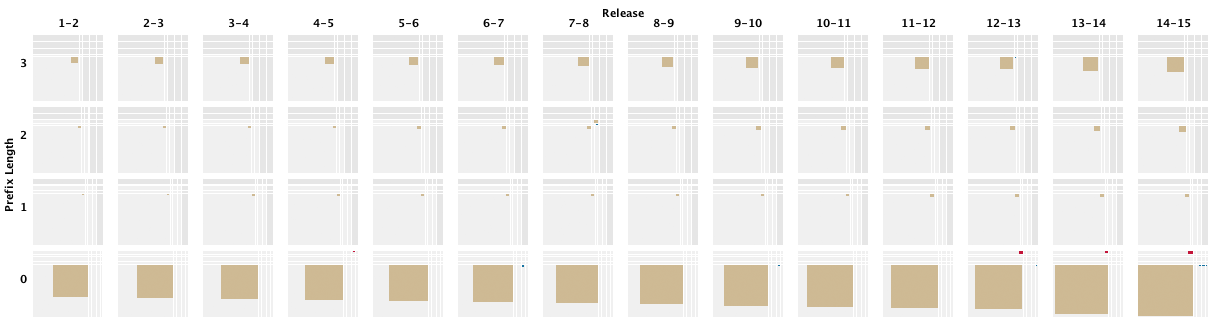
\includegraphics[width=17cm]{images/squaremap011.png}
  \caption{Normal scale, Stable entries + changes, Global normalization}
  \label{fig:heatmap011}
\end{figure*}

\begin{figure*}[htb]
  \centering
  %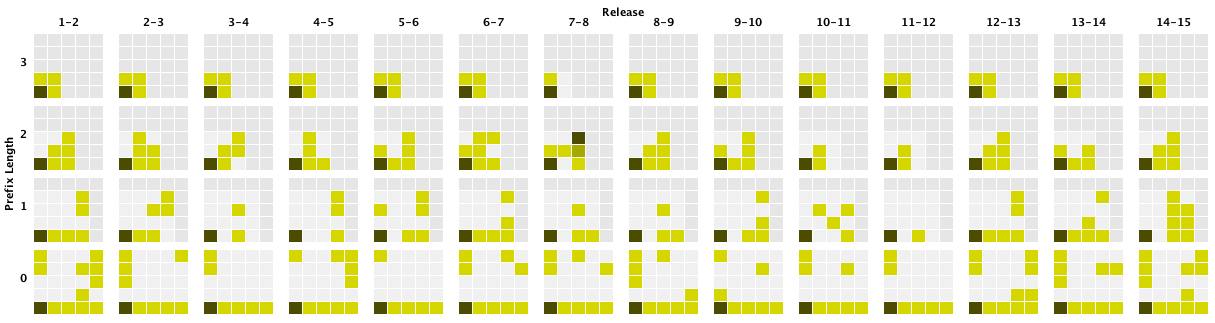
\includegraphics[width=17cm]{images/heatmap010.png}
  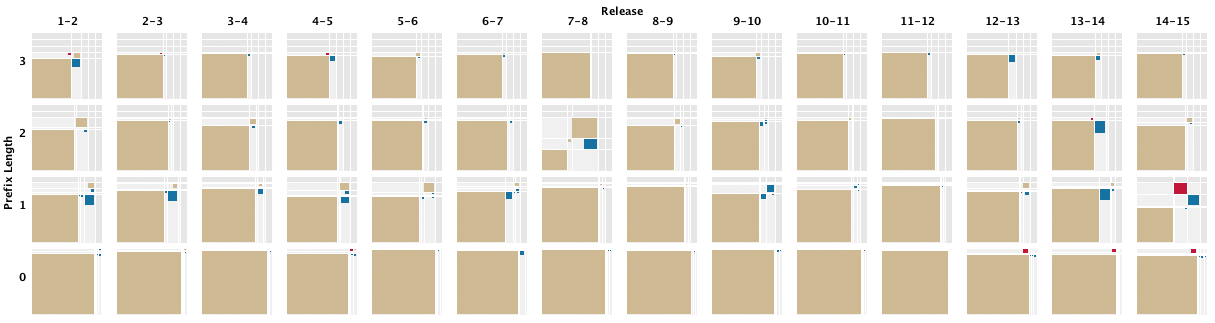
\includegraphics[width=17cm]{images/squaremap010.png}
  \caption{Normal scale, Stable entries + changes, Local normalization}
  \label{fig:heatmap010}
\end{figure*}

\subsubsection{Generalization versus Specialization}

%Consider, for each frame, a diagonal that extends from the bottom left corner to the top right corner. The matrix of points below this diagonal, called lower right triangular matrix, represents changes in which there are more specializations than generalizations. In a similar manner, the matrix of points above this diagonal, called upper left triangular matrix, represents changes in which there are more generalizations than specializations. In Heatmaps of Figure \ref{fig:heatmap010} and \ref{fig:heatmap011}, for instance, the lower triangular matrices have more points than the superior ones, and therefore in the entire data set there are more specializations than generalizations. In Figure \ref{fig:heatmap000}, where we present only changes in normal scale and local normalization, we can see a predominance of blue rectangles representing this trend. Once again, exceptions are evidenced as some are going to be discussed further in \ref{sec:exceptions}.

Consider, for each frame, a diagonal that extends from the bottom left corner to the top right corner. The matrix of subframes below this diagonal, called lower right triangular matrix, is composed of changes in which there were more specializations than generalizations. In a similar manner, the matrix of subframes above this diagonal, called upper left triangular matrix, is composed of changes in which there were more generalizations than specializations. In the Heatmap of Figure \ref{fig:heatmap000}, for exaple, the lower triangular matrices have more entries than the superior ones and, this, in the entire data set there were more specializations than generalizations. In Figure \ref{fig:heatmap000}, where we present only changes in linear scale and local normalization, we can see a predominance of blue rectangles representing this trend. Once again, exceptions are evidenced and some of them are going to be discussed further in \ref{sec:exceptions}.

\begin{figure*}[htb]
  \centering
  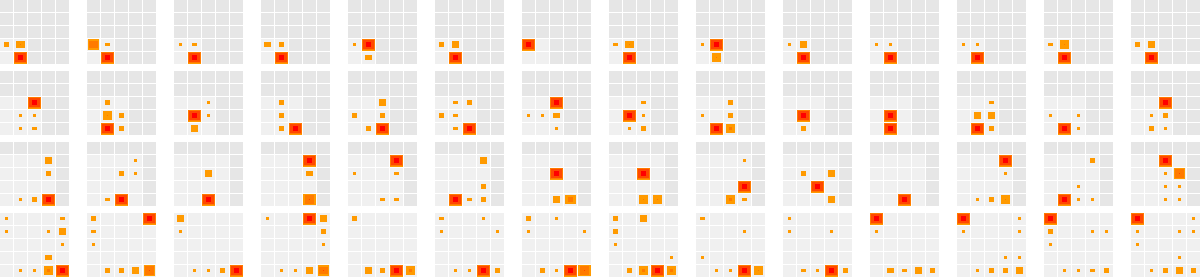
\includegraphics[width=17cm]{images/heatmap000.png}     
  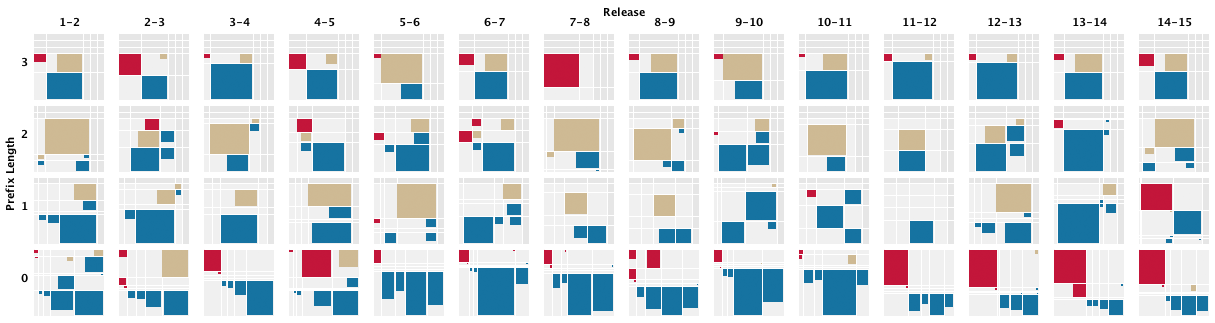
\includegraphics[width=17cm]{images/squaremap000.png}
  \caption{Normal scale, Only changes, Local normalization}
  \label{fig:heatmap000}
\end{figure*}

%In Figure \ref{fig:heatmap100}, we represent only changes in log scale and local normalization. It emphasizes that line representing 0 generalizations from last line of multivariate matrix (common prefix length) a frequent change type. It reveals an interesting trend of specialization of entries without annotation (-.-.-.-) as they tend to get annotations along all the releases.

Figure \ref{fig:heatmap000} also emphasizes that the line representing no generalizations in the bottom row of frames (common prefix length 0) in the multivariate matrix is a frequent type of change. It reveals an interesting trend of specialization for entries without annotation (-.-.-.-) as they tend to receive EC levels in each releases.

%\begin{figure*}[htb]
%  \centering
%  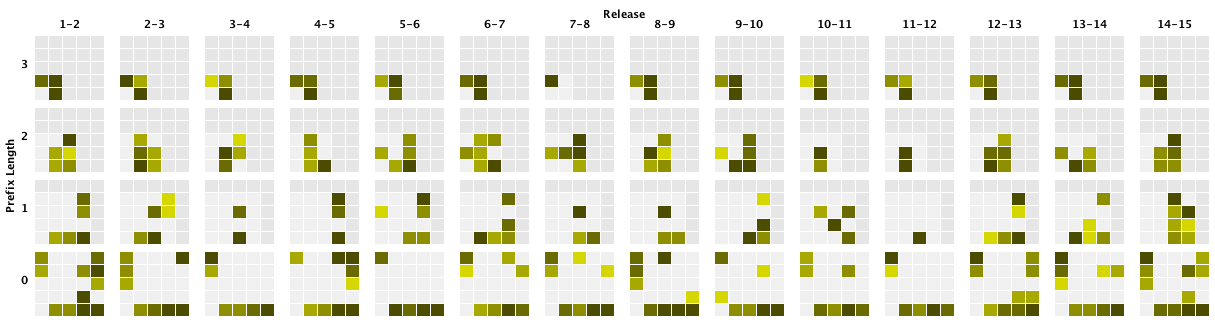
\includegraphics[width=17cm]{images/heatmap100.png} 
%  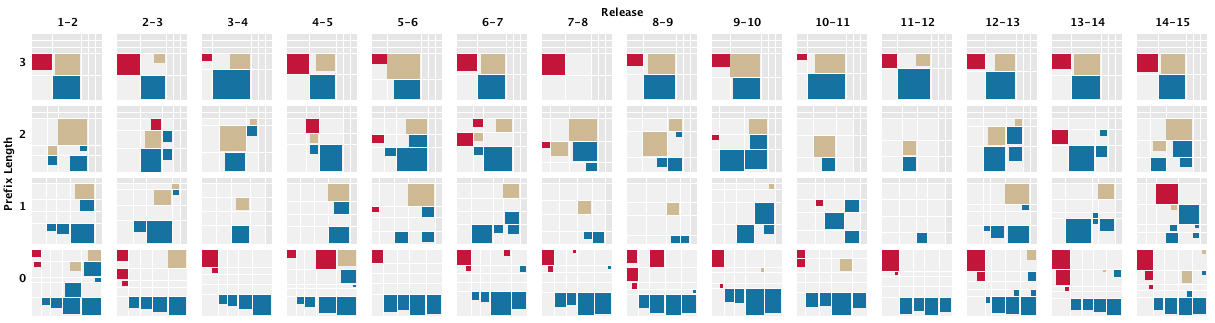
\includegraphics[width=17cm]{images/squaremap100.png}
%  \caption{Log scale, Only changes, Local normalization}
%  \label{fig:heatmap100}
%\end{figure*}

\subsection{Exceptions} 
\label{sec:exceptions}

%Falar que nas versões 11 a 15 foram identificadas mudanças drásticas bem numerosas (deleções de 4 níveis). Colocar quantas entradas sofreram tais mudanças. Colocar exemplos biológicos do que isso significa (de acordo com a resposta do UniProt).

\subsubsection{Annotation deletion}

The four subframes, spotted by their red rectangles on the bottom row of figure \ref{fig:heatmap001}, that the parameters are common prefix length 0, 4 degress of generalization and no specialization, in releases 12-13, 13-14 and 14-15, represent a drastic change in which the four levels of involved EC numbers were deleted. The table \ref{four_deletion} shows the frequencies related to each subframe.

\begin{figure*}[htb]
  \centering
  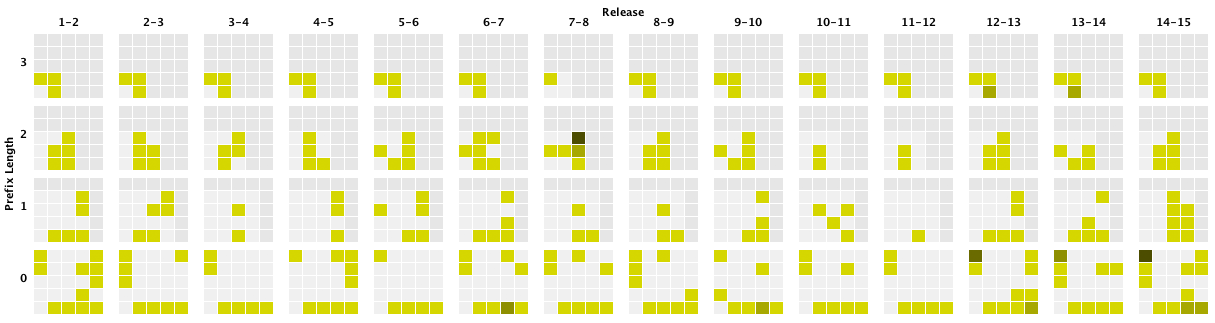
\includegraphics[width=17cm]{images/heatmap001.png}  
  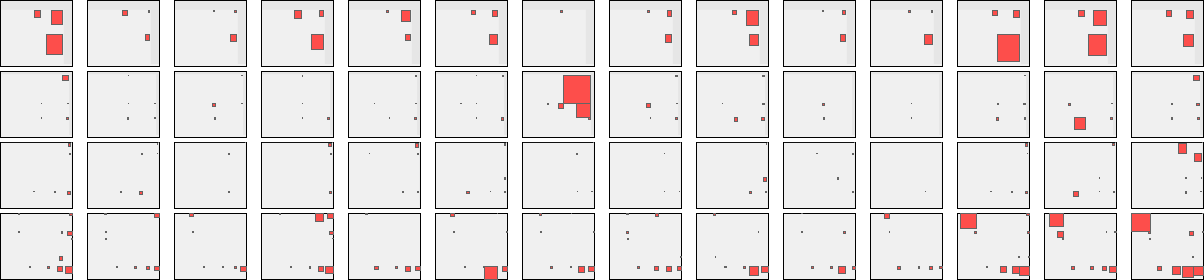
\includegraphics[width=17cm]{images/squaremap001.png}
  \caption{Normal scale, Only changes, Global normalization}
  \label{fig:heatmap001}
\end{figure*}

\begin{table}[!h]
  \caption{Frequency of four-level EC number deletion from releases 11 to 15}
  \label{four_deletion}
  \scriptsize
  \begin{center}
    \begin{tabular}{cccc}
      Pair of releases & Frequencies\\
    \hline
      11-12 & 146\\
      12-13 &  1,357\\
      13-14 & 1,006\\
      14-15 & 1,976
    \end{tabular}
  \end{center}
\end{table}

EC numbers must be assigned to protein catalytic subunits. This implies that in large protein complexes only one or a few of the subunits will be annotated with an EC number. Indeed, proteins can have non catalytical functions like transport of substances, immunological or structural. In some cases, automatic annotation can assign EC numbers to a whole complex with non-catalytic subunits. Subframes that symbolize such cases in ADVISe represent corrections where the curators completely removed the EC numbers since the concerned subunits are not enzymes. We present three examples of UniProt/SwissProt entries that experienced four-level EC number deletion from releases 12 to 13. 

\begin{itemize}
\item Identifier Q6FSJ2, which was annotated as 1.10.2.2 in version 12, is subunit 7 of Cytochrome b-c1, but not the subunit with Reductase Activity
\item Identifier Q8LX28, whose annotation was 3.6.3.14 in version 12, is subunit 8 of ATP Synthase, which is part of the membrane proton channel
\item Identifier Q6AY96, which was annotated as 2.7.11.1 in version 12, is a subunit of a transcription factor, but not the subunit with Serine/Threonine Kinase activity.
\end{itemize}

\subsubsection{Deleted EC numbers}

In Figure \ref{fig:heatmap001}, the subframe with common prefix length 0, 2 degrees of generalization and 2 degrees of specialization in releases 7 to 8, a total of 1,900 EC number changes are represented. The three most numerous changes depicted in this subframe are, respectively, 2.7.1.37 to 2.7.11.1 (918 entries), 2.7.1.112 to 2.7.10.1 (215 entries) and 2.7.1.112 to 2.7.10.2 (165 entries). As stated by IUBMB, the EC number 2.7.1.37 was deleted and divided in 2005 into 2.7.11.1, 2.7.11.8, 2.7.11.9, 2.7.11.10, 2.7.11.11, 2.7.11.12, 2.7.11.13, 2.7.11.21, 2.7.11.22, 2.7.11.24, 2.7.11.25, 2.7.11.30 and 2.7.12.1. The same happened to the EC number 2.7.1.112, that was deleted and divided into 2.7.10.1 and 2.7.10.2. In such cases, Transferase annotations, more specifically 2.7.*.* (transferring phosphorus-containing groups), underwent a revision caused by a change in the Enzyme Classification system, not by a change in enzyme function annotation.

Something similar happened in the subframe with common prefix length 1, 2 degrees of generalization and 3 degrees of specialization in releases 14 to 15 (212 entries). This subframe can be better visualized in the Quadmap of figure \ref{fig:heatmap001} and it represents the EC number change 2.5.1.- (transferring alkyl or aryl groups, other than methyl groups) to 2.2.1.9 (2-succinyl-5-enolpyruvyl-6-hydroxy-3-cyclohexene-1-carboxylic-acid synthase). The EC number 2.5.1.64 was created in 2003 and deleted in 2008 when it was divided into 2.2.1.9 and 4.2.99.20. In this case, the annotation changes are due to the creation of a new EC (2.2.1.9), in other words, there was a change in the Enzyme Classification system.

\subsubsection{Created EC numbers}

In some cases, enzymes were integrated to UniProt/SwissProt when their catalytic activity was already known but there were no appropriate EC numbers defined by IUBMB to describe such catalytic activity . For example, in Figure \ref{fig:heatmap001}, the subframe with parameters common prefix length 3, no generalizations and 1 degree of specialization in releases 12 to 13, represents a total of 637 EC number changes. A representative EC number change depicted by this subframe is from 2.8.1.- (sulfurtransferases) to 2.8.1.8 (EC created in 2006 to represent lipoyl synthase), with 117 entries. The UniProt entry Q7UH37 suffered this change. It was integrated to UniProt in 10 May 2004 and its associated function was lipoyl synthase. However, there was not an EC number related to lipoyl synthase at that moment and this entry remained with the same incomplete EC number 2.8.1.- until release 13 (26 Feb 2008), when it was annotated with EC number 2.8.1.8.

\subsubsection{Annotation errors}

Another exception we detected is presented in Figure \ref{fig:heatmap001} by the red subframe with parameters common prefix length 1, 3 degrees of generalization and 2 degrees of specialization in releases 14 to 15. This subframe represents a single kind of change which happened 261 times. The EC number change was from 2.1.1.61, which was created in 1982 and associated with tRNA (5-methylaminomethyl-2-thiouridylate-methyltransferase) function, to 2.8.1.-, which is associated with sulfurtransferase function. The EC number 2.1.1.61 was not deleted, so the EC number change was a correction in order to annotate the involved entries with a more approprite catalytic function.



